\section{Application-level conventions}\label{sec:application_level_conventions}

This section describes a set of high-level conventions designed to enhance compatibility
of applications leveraging UAVCAN.
The conventions described here are not mandatory to follow;
however, every deviation should be justified and documented.

\subsection{Node identifier distribution}

An overview of related concepts is provided in chapter \ref{sec:basic_concepts}.

Valid values of node-ID range from 0 up to a transport-specific upper boundary
which is guaranteed to be above 127 for any transport.

The two uppermost node-ID values are reserved for diagnostic and debugging tools;
these node-ID values should not be used in fielded systems.

\subsection{Timing constraints}

\subsubsection{Recommended message publication timing constraints}

Generally, it is recommended to abort a message transmission if it cannot be completed in 1 second.

It is expected that high-frequency high-priority messages may opt for lower timeout values,
whereas low-priority delayable data may opt for higher timeout values to account for network congestion.
Refer to section \ref{sec:transport_transfer_priority} on transfer prioritization.

\subsubsection{Recommended service invocation timing constraints}

It is recommended to abort a service transfer transmission if it cannot be completed in 1 second.
It is recommended to stop waiting for a service response if it could not be received in the same amount of time;
upon reaching this condition, the service request operation should be considered unsuccessful.

If the server uses a significant part of the timeout period to process the request,
the client might drop the request before receiving the response.
It is recommended to ensure that the server will be able to process any request in less than 0.5 seconds.

\subsection{Coordinate frames}

UAVCAN follows the conventions that are widely accepted in relevant applications.
Adherence to the coordinate frame conventions described here maximizes compatibility and
reduces the amount of computations for conversions between incompatible coordinate systems and
representations.
It is recognized, however, that some applications may find the advised conventions unsuitable,
in which case deviations are permitted.
Any such deviations shall be explicitly documented.

All coordinate systems defined in this section are right-handed.
If application-specific coordinate systems are introduced, they should be right-handed as well.

\begin{figure}[hbt]
    \centering
    % The source image is released under CC0, public domain, no attribution required:
    % https://commons.wikimedia.org/wiki/File:ECEF_ENU_Longitude_Latitude_relationships.svg
	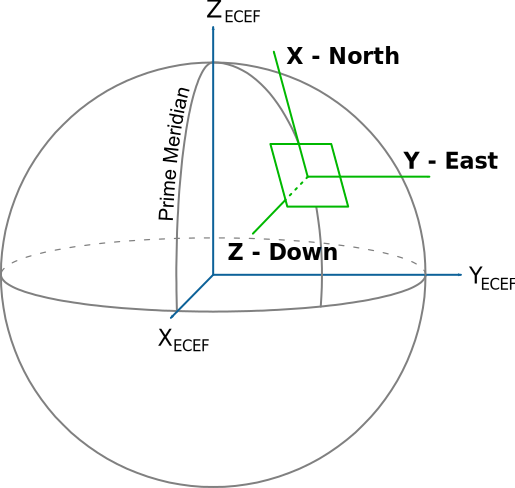
\includegraphics[width=0.45\textwidth]{application_layer/NED_ECEF}
    % The source image is released under CC0, public domain, no attribution required:
    % https://pixabay.com/en/airplane-plane-aircraft-propeller-40374/
    % The final image is drawn by me. The source Inkscape SVG file is located in the same directory.
    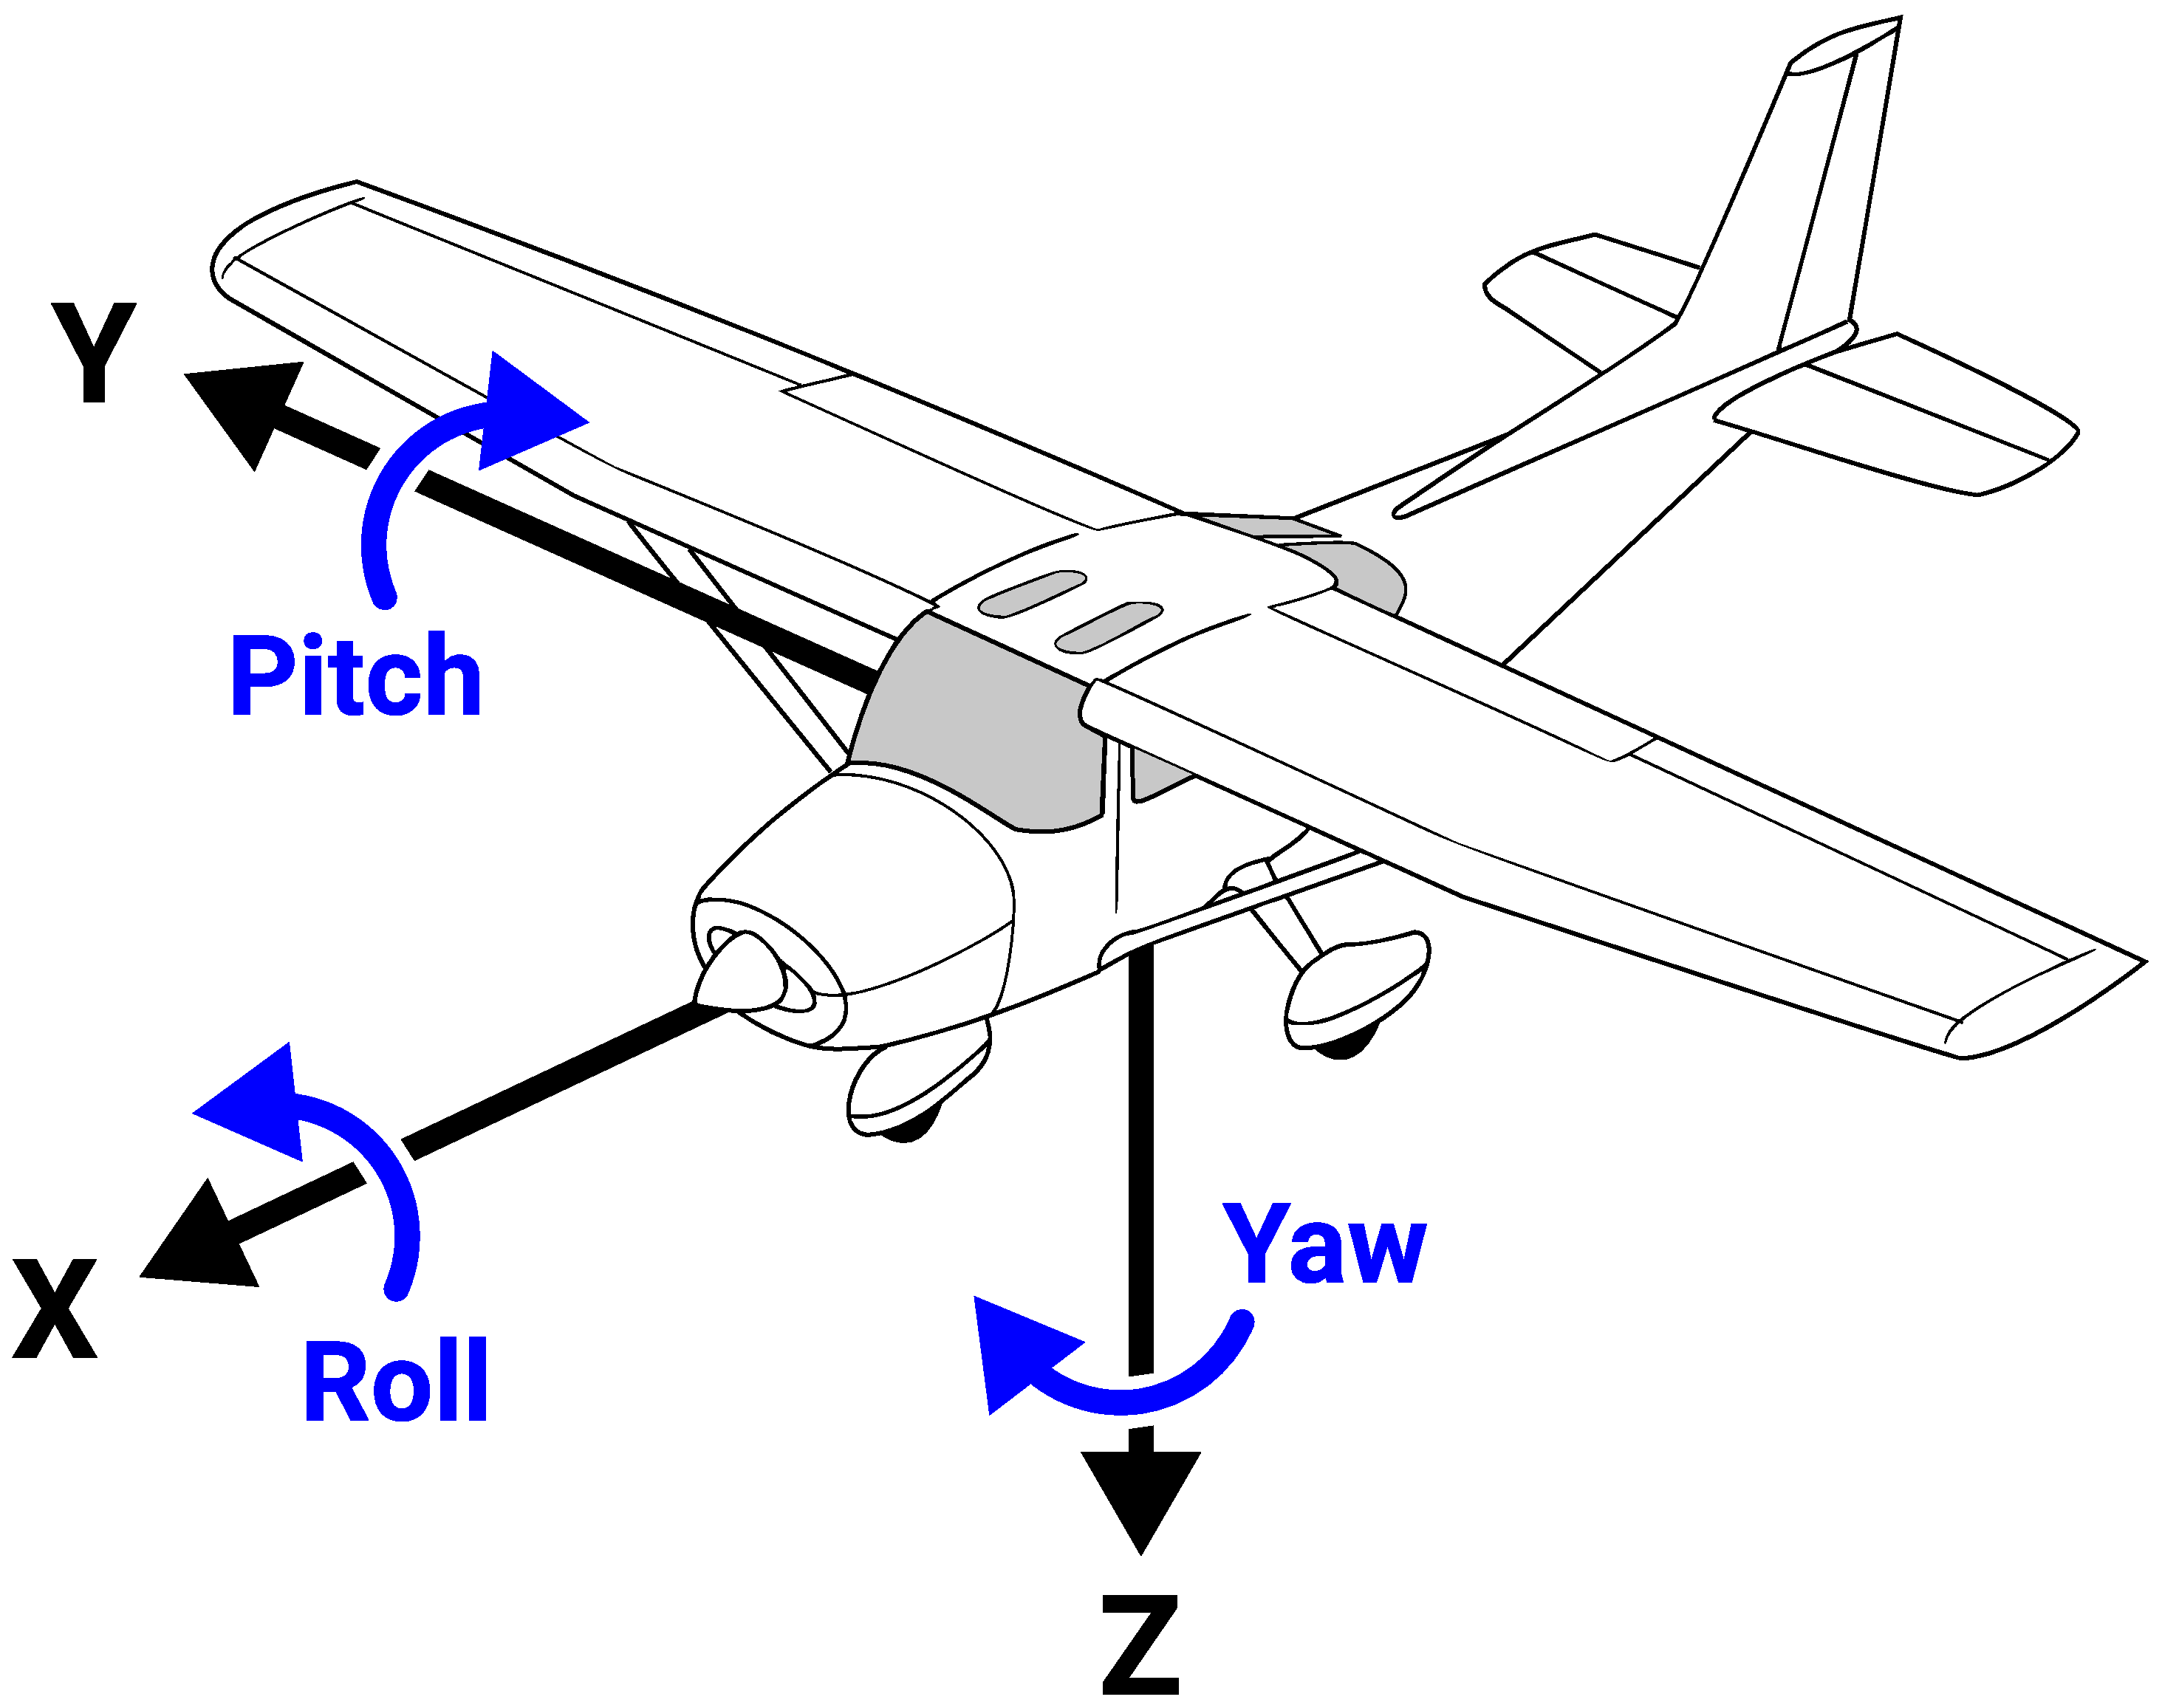
\includegraphics[width=0.45\textwidth]{application_layer/aircraft_principal_axes}
    North-East-Down (NED) frame and body frame conventions. All systems are right-handed.
    \caption{
        Coordinate frame conventions.
        \label{fig:application_coordinate_frame_conventions}
    }
\end{figure}

\subsubsection{World frame}

For world fixed frames, the \emph{North-East-Down} (NED) right-handed notation is preferred.
\begin{samepage}
\begin{description}
    \item[X] --- northward;
    \item[Y] --- eastward;
    \item[Z] --- down.
\end{description}
\end{samepage}

\subsubsection{Body frame}

In relation to a body, the convention is as defined below, right-handed.
This convention is widely used in aeronautic applications.
\begin{samepage}
\begin{description}
    \item[X] --- forward;
    \item[Y] --- right;
    \item[Z] --- down.
\end{description}
\end{samepage}

\subsubsection{Optical frame}

In the case of cameras, the right-handed convention specified below is preferred.
It is widely used in various applications involving computer vision systems.
\begin{samepage}
\begin{description}
    \item[X] --- right;
    \item[Y] --- down;
    \item[Z] --- towards the scene along the optical axis.
\end{description}
\end{samepage}

\subsection{Rotation representation}

All applications should represent rotations using quaternions with the elements ordered as follows\footnote{%
    Assuming $w + x\boldsymbol{i} + y\boldsymbol{j} + z\boldsymbol{k}$.
}: W, X, Y, Z.
Other forms of rotation representation should be avoided.

Angular velocities should be represented using the right-handed, fixed-axis (extrinsic) convention:
X (roll), Y (pitch), Z (yaw).

\begin{remark}
    Quaternions are considered to offer the optimal trade-off between bandwidth efficiency,
    computation complexity, and explicitness:
    \begin{itemize}
        \item Euler angles are not self-contained, requiring applications to agree on a particular
        convention beforehand; a convention would be difficult to establish considering different
        demands of various use cases.

        \item Euler angles and fixed axis rotations typically cannot be used for computations directly
        due to angular interpolation issues and singularities; thus, to make use of such
        representations, one often has to convert them to a different form (e.g., quaternion);
        such conversions are computationally heavy.

        \item Rotation matrices are highly redundant.
    \end{itemize}
\end{remark}

\subsection{Matrix representation}

\subsubsection{General}

Matrices should be represented as flat arrays in the row-major order.

\begin{remark}
    $
    \begin{bmatrix}
        x_{11} & x_{12} & x_{13} \\
        x_{21} & x_{22} & x_{23} \\
    \end{bmatrix} \rightarrow \left(x_{11}, x_{12}, x_{13}, x_{21}, x_{22}, x_{23}\right)
    $
\end{remark}

\subsubsection{Square matrices}

There are standard compressed representations of an $n \times n$ square matrix.

An array of size $n^2$ represents a full square matrix.
This is equivalent to the general case reviewed above.

An array of $\frac{(1 + n) n}{2}$ elements represents a symmetric matrix,
where array members represent the elements of the upper-right triangle arranged in the row-major order.
\begin{remark}
    $
    \begin{bmatrix}
        a & b & c \\
        b & d & e \\
        c & e & f \\
    \end{bmatrix} \rightarrow \left(a, b, c, d, e, f\right)
    $

    This form is well-suited for covariance matrix representation.
\end{remark}

An array of $n$ elements represents a diagonal matrix,
where an array member at position $i$ (where $i=1$ for the first element)
represents the matrix element $x_{i, i}$ (where $x_{1, 1}$ is the upper-left element).
\begin{remark}
    $
    \begin{bmatrix}
        a & 0 & 0 \\
        0 & b & 0 \\
        0 & 0 & c \\
    \end{bmatrix} \rightarrow \left(a, b, c\right)
    $
\end{remark}

An array of one element represents a scalar matrix.
\begin{remark}
    $
    \begin{bmatrix}
        a & 0 & 0 \\
        0 & a & 0 \\
        0 & 0 & a \\
    \end{bmatrix} \rightarrow a
    $
\end{remark}

An empty array represents a zero matrix.

\subsubsection{Covariance matrices}

A zero covariance matrix represents an unknown covariance\footnote{%
    As described above, an empty array represents a zero matrix,
    from which follows that an empty array represents unknown covariance.
}.

Infinite error variance means that the associated value is undefined.

\subsection{Physical quantity representation}

\subsubsection{Units}

All units should be SI\footnote{International System of Units.} units (base or derived).
Usage of any other units is strongly discouraged.

When defining data types, fields and constants that represent unscaled quantities in SI units
should not have suffixes indicating the unit, since that would be redundant.

On the other hand, fields and constants that contain quantities in
non-SI units\footnote{E.g., degree Celsius instead of kelvin.}
or scaled SI units\footnote{E.g., microsecond instead of second.}
should be suffixed with the standard abbreviation of the unit\footnote{E.g., kg for kilogram, J for joule.}
and its metric prefix\footnote{E.g., M for mega, n for nano.}
(if any), maintaining the proper letter case of the abbreviation.
In other words, the letter case of the suffix is independent of the letter case of
the attribute it is attached to.

Scaling coefficients should not be chosen arbitrarily;
instead, the choice should be limited to the standard metric prefixes defined by the
International System of Units.

All standard metric prefixes have well-defined abbreviations that are constructed from ASCII characters,
except for one: the micro prefix is abbreviated as a Greek letter ``\textmu{}'' (mu).
When defining data types, ``\textmu{}'' should be replaced with the lowercase Latin letter ``u''.

Irrespective of the suffix, it is recommended to always specify units for every field in the comments.

\begin{remark}
    \begin{minted}{python}
        float16 temperature           # [kelvin] Suffix not needed because an unscaled SI unit is used here.

        uint24 delay_us               # [microsecond] Scaled SI unit, suffix required. Mu replaced with "u".
        uint24 MAX_DELAY_us = 600000  # [microsecond] Notice the letter case.

        float32 kinetic_energy_GJ     # [gigajoule] Notice the letter case.

        float16 estimated_charge_mAh  # [milliampere hour] Scaled non-SI unit. Discouraged, use coulomb.
        float16 MAX_CHARGE_mAh = 1e4  # [milliampere hour] Notice the letter case.
    \end{minted}
\end{remark}

\subsubsection{Enhanced type safety}

It is recommended to avoid reliance on raw scalar types (such as \verb|float32|)
when defining fields containing physical quantities.
Instead, the explicitly typed alternatives defined in the standard DSDL namespace
\DSDLReference{uavcan.si.unit} (also see section \ref{sec:application_si}) should be used.

\begin{remark}
    \begin{minted}{python}
        # Kinetic energy of four bodies.
        float32[4] kinetic_energy                           # [joule] Not recommended.
        uavcan.si.unit.energy.Scalar.1.0[4] kinetic_energy  # This is the recommended practice.

        # 3D velocity vector.
        float32[3] velocity                                 # [meter/second] Not recommended.
        uavcan.si.unit.velocity.Vector3.1.0                 # This is the recommended practice.
    \end{minted}
\end{remark}
